\documentclass[11pt,a4paper]{article}

\usepackage[margin=1.5cm]{geometry}
\usepackage{tikz}
\usetikzlibrary{shapes.geometric, arrows.meta, positioning, fit, backgrounds, shadows.blur}
\usepackage{xcolor}
\usepackage[T1]{fontenc}
\usepackage{amsmath}

% ── Colour palette ────────────────────────────────────────────────────────
\definecolor{startend}{RGB}{0,70,140}
\definecolor{process}{RGB}{30,120,200}
\definecolor{decision}{RGB}{0,130,80}
\definecolor{output}{RGB}{160,50,30}
\definecolor{solver}{RGB}{100,30,130}
\definecolor{textwhite}{RGB}{255,255,255}
\definecolor{arrowgray}{RGB}{80,80,80}

% ── TikZ styles ───────────────────────────────────────────────────────────
\tikzset{
  % Terminal (start/end)
  terminal/.style={
    rectangle, rounded corners=12pt,
    minimum width=5.2cm, minimum height=0.85cm,
    fill=startend, draw=startend!80!black, line width=0.8pt,
    text=textwhite, font=\bfseries\small, align=center
  },
  % Process box
  process/.style={
    rectangle, rounded corners=4pt,
    minimum width=5.2cm, minimum height=0.85cm,
    fill=process, draw=process!80!black, line width=0.6pt,
    text=textwhite, font=\small, align=center
  },
  % Subprocess (indented / narrower)
  subprocess/.style={
    rectangle, rounded corners=3pt,
    minimum width=4.6cm, minimum height=0.75cm,
    fill=process!70!white, draw=process!80!black, line width=0.5pt,
    text=process!20!black, font=\footnotesize, align=center
  },
  % Decision diamond
  decision/.style={
    diamond, aspect=2.8,
    minimum width=5.6cm, minimum height=1.1cm,
    fill=decision, draw=decision!80!black, line width=0.7pt,
    text=textwhite, font=\small\bfseries, align=center, inner sep=0pt
  },
  % Solver block
  solverbox/.style={
    rectangle, rounded corners=4pt,
    minimum width=5.2cm, minimum height=0.85cm,
    fill=solver, draw=solver!80!black, line width=0.6pt,
    text=textwhite, font=\small, align=center
  },
  % Output block
  outputbox/.style={
    rectangle, rounded corners=4pt,
    minimum width=5.2cm, minimum height=0.85cm,
    fill=output, draw=output!80!black, line width=0.6pt,
    text=textwhite, font=\small, align=center
  },
  % Arrow style
  arr/.style={
    -Stealth, thick, color=arrowgray, line width=1pt
  },
  % Thin dashed back-arrow
  backarr/.style={
    -Stealth, dashed, color=arrowgray!70, line width=0.7pt
  },
  % Side label
  sidelabel/.style={
    font=\footnotesize\itshape, text=arrowgray
  },
}

\begin{document}
\pagestyle{empty}

% ─────────────────────────────────────────────────────────────────────────
\begin{center}
  {\Large\bfseries\color{startend}
   Notebook Manufacturing Scheduling\\[3pt]
   Optimization Pipeline --- Flowchart}
\end{center}
\vspace{4pt}
\hrule
\vspace{10pt}

\begin{center}
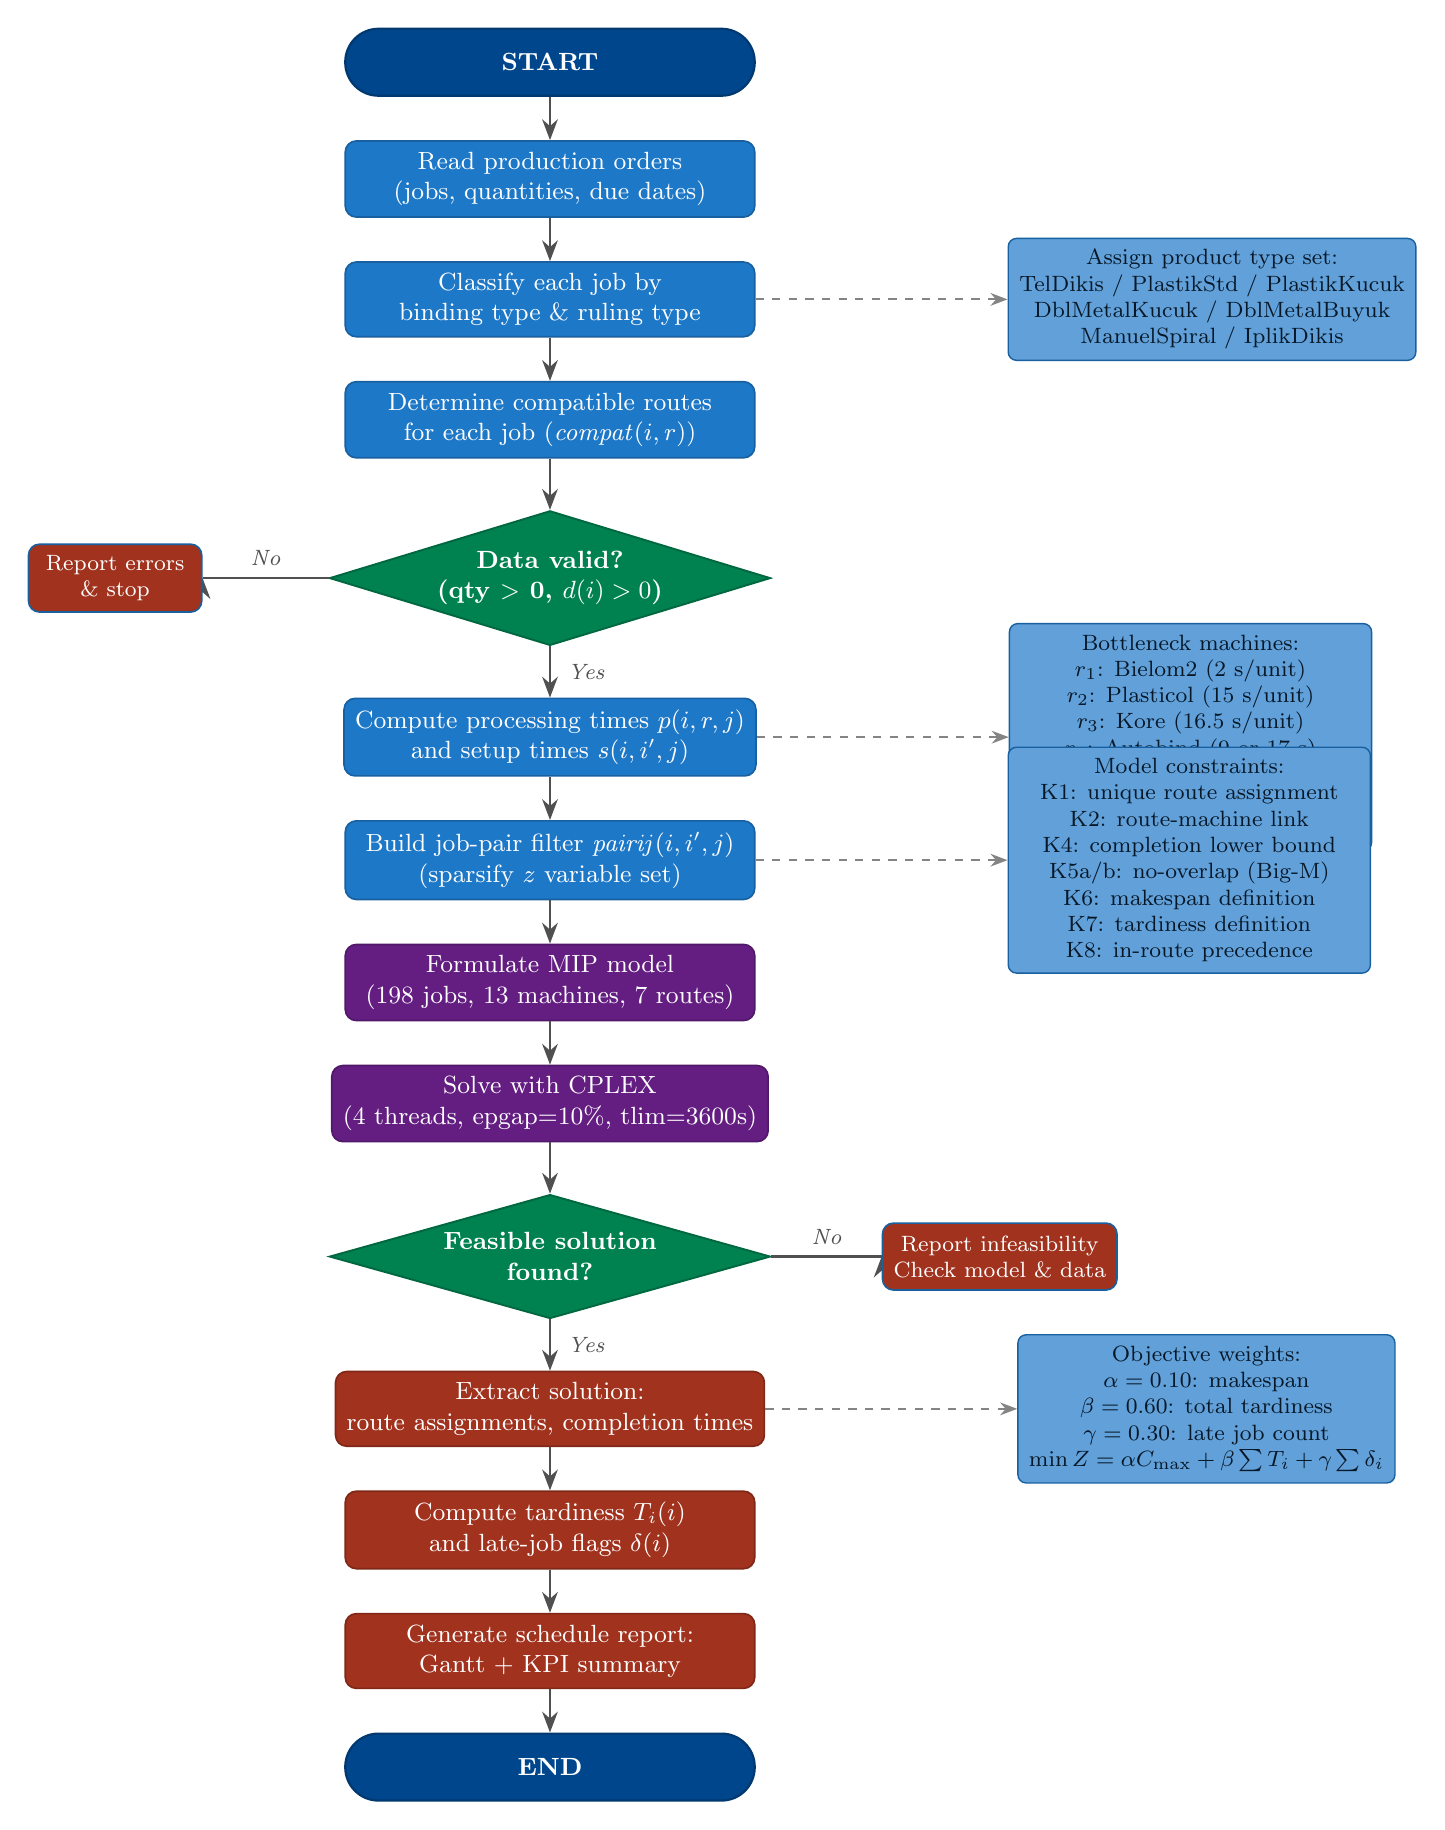
\begin{tikzpicture}[
  node distance=0.55cm and 3.2cm,
  every node/.style={inner sep=4pt}
]

%% ── COLUMN 1 (main flow) ─────────────────────────────────────────────────

\node[terminal] (start) {START};

\node[process, below=of start]  (input)
  {Read production orders\\(jobs, quantities, due dates)};

\node[process, below=of input]  (classify)
  {Classify each job by\\binding type \& ruling type};

\node[process, below=of classify] (route)
  {Determine compatible routes\\for each job ($\mathit{compat}(i,r)$)};

\node[decision, below=0.65cm of route] (valid)
  {Data valid?\\(qty $>$ 0, $d(i)>0$)};

\node[process, below=0.65cm of valid]  (param)
  {Compute processing times $p(i,r,j)$\\and setup times $s(i,i',j)$};

\node[process, below=of param]  (pairs)
  {Build job-pair filter $\mathit{pairij}(i,i',j)$\\(sparsify $z$ variable set)};

\node[solverbox, below=of pairs] (mip)
  {Formulate MIP model\\(198 jobs, 13 machines, 7 routes)};

\node[solverbox, below=of mip]  (cplex)
  {Solve with CPLEX\\(4 threads, epgap=10\%, tlim=3600s)};

\node[decision, below=0.65cm of cplex] (feasible)
  {Feasible solution\\found?};

\node[outputbox, below=0.65cm of feasible] (extract)
  {Extract solution:\\route assignments, completion times};

\node[outputbox, below=of extract] (tardiness)
  {Compute tardiness $T_i(i)$\\and late-job flags $\delta(i)$};

\node[outputbox, below=of tardiness] (report)
  {Generate schedule report:\\Gantt + KPI summary};

\node[terminal, below=of report] (end) {END};

%% ── COLUMN 2 (side processes: parameter detail) ──────────────────────────

\node[subprocess, right=3.2cm of classify] (prodtype)
  {Assign product type set:\\TelDikis / PlastikStd / PlastikKucuk\\DblMetalKucuk / DblMetalBuyuk\\ManuelSpiral / IplikDikis};

\node[subprocess, right=3.2cm of param] (bottleneck)
  {Bottleneck machines:\\$r_1$: Bielom2 (2 s/unit)\\$r_2$: Plasticol (15 s/unit)\\$r_3$: Kore (16.5 s/unit)\\$r_4$: Autobind (9 or 17 s)\\$r_5$: CWH (15 or 23 s)\\$r_6$: ManSpiral (17 s)\\$r_7$: Juki (15 s)};

\node[subprocess, right=3.2cm of pairs] (constraints)
  {Model constraints:\\K1: unique route assignment\\K2: route-machine link\\K4: completion lower bound\\K5a/b: no-overlap (Big-M)\\K6: makespan definition\\K7: tardiness definition\\K8: in-route precedence};

\node[subprocess, right=3.2cm of extract] (objective)
  {Objective weights:\\$\alpha=0.10$: makespan\\$\beta=0.60$: total tardiness\\$\gamma=0.30$: late job count\\$\min Z = \alpha C_{\max} + \beta\sum T_i + \gamma\sum\delta_i$};

%% ── MAIN ARROWS ──────────────────────────────────────────────────────────

\draw[arr] (start)     -- (input);
\draw[arr] (input)     -- (classify);
\draw[arr] (classify)  -- (route);
\draw[arr] (route)     -- (valid);
\draw[arr] (valid)     -- node[sidelabel, right=2pt]{Yes} (param);
\draw[arr] (param)     -- (pairs);
\draw[arr] (pairs)     -- (mip);
\draw[arr] (mip)       -- (cplex);
\draw[arr] (cplex)     -- (feasible);
\draw[arr] (feasible)  -- node[sidelabel, right=2pt]{Yes} (extract);
\draw[arr] (extract)   -- (tardiness);
\draw[arr] (tardiness) -- (report);
\draw[arr] (report)    -- (end);

%% ── DECISION BRANCHES (No paths) ─────────────────────────────────────────

% "Data not valid" → exit left
\draw[arr] (valid.west) -- ++(-1.6,0)
    node[sidelabel, above, midway]{No}
    node[process, left, minimum width=2.2cm, font=\footnotesize, fill=output]{Report errors\\\& stop}
    ($(valid.west)+(-1.6,0)$);

% "Not feasible" → report infeasibility
\draw[arr] (feasible.east) -- ++(1.4,0)
    node[sidelabel, above, midway]{No}
    node[process, right, minimum width=2.6cm, font=\footnotesize, fill=output]{Report infeasibility\\Check model \& data}
    ($(feasible.east)+(1.4,0)$);

%% ── SIDE CONNECTOR ARROWS ────────────────────────────────────────────────

\draw[backarr] (classify.east) -- (prodtype.west);
\draw[backarr] (param.east)    -- (bottleneck.west);
\draw[backarr] (pairs.east)    -- (constraints.west);
\draw[backarr] (extract.east)  -- (objective.west);

\end{tikzpicture}
\end{center}

\vspace{8pt}
\hrule
\vspace{6pt}

% ── Legend ────────────────────────────────────────────────────────────────
\begin{center}

\begin{tikzpicture}
  \node[terminal, minimum width=2.6cm, minimum height=0.6cm, font=\footnotesize] (l1) {Start / End};
  \node[process,  minimum width=2.6cm, minimum height=0.6cm, font=\footnotesize,
        right=0.5cm of l1] (l2) {Process step};
  \node[decision, minimum width=2.8cm, minimum height=0.7cm, font=\footnotesize,
        right=0.5cm of l2] (l3) {Decision};
  \node[solverbox, minimum width=2.6cm, minimum height=0.6cm, font=\footnotesize,
        right=0.5cm of l3] (l4) {MIP / Solver};
  \node[outputbox, minimum width=2.6cm, minimum height=0.6cm, font=\footnotesize,
        right=0.5cm of l4] (l5) {Output / Report};
  \node[subprocess, minimum width=2.6cm, minimum height=0.6cm, font=\footnotesize,
        right=0.5cm of l5] (l6) {Detail panel};
\end{tikzpicture}
\end{center}

\end{document}
